\documentclass[11pt,a4paper]{article}

% ── packages ────────────────────────────────────────────────────────────────
\usepackage[a4paper, margin=2.5cm, headheight=15pt]{geometry}
\usepackage{fontenc}
\usepackage{inputenc}
\usepackage{microtype}
\usepackage{graphicx}
\usepackage{booktabs}
\usepackage{colortbl}
\usepackage{tabularx}
\usepackage{array}
\usepackage{multirow}
\usepackage{amsmath}
\usepackage{amssymb}
\usepackage{xcolor}
\usepackage{hyperref}
\usepackage{titlesec}
\usepackage{enumitem}
\usepackage{caption}
\usepackage{subcaption}
\usepackage{fancyhdr}
\usepackage{tcolorbox}
\usepackage{float}
\usepackage{parskip}
\usepackage{mdframed}
\usepackage{tikz}
\usepackage{pgfplots}
\pgfplotsset{compat=1.18}
\usepackage{listings}
\usepackage{inconsolata}
\lstset{
  language=Python,
  basicstyle=\ttfamily\footnotesize,
  keywordstyle=\bfseries\color{accent},
  commentstyle=\itshape\color{gray},
  stringstyle=\color{orange},
  numbers=left,
  numberstyle=\tiny\color{gray},
  numbersep=6pt,
  breaklines=true,
  frame=single,
  rulecolor=\color{rulecol},
  backgroundcolor=\color{accentlight!30},
  xleftmargin=12pt,
  framexleftmargin=12pt,
  showstringspaces=false,
  tabsize=4,
  morekeywords={F,nn,torch,self},
}

% ── colours ─────────────────────────────────────────────────────────────────
\definecolor{accent}{RGB}{30,100,200}
\definecolor{accentlight}{RGB}{220,232,255}
\definecolor{tableheadbg}{RGB}{30,60,120}
\definecolor{rowodd}{RGB}{245,248,255}
\definecolor{roweven}{RGB}{255,255,255}
\definecolor{green}{RGB}{39,174,96}
\definecolor{orange}{RGB}{230,126,34}
\definecolor{gray}{RGB}{100,110,130}
\definecolor{lightgray}{RGB}{230,235,245}
\definecolor{darktext}{RGB}{20,30,50}
\definecolor{rulecol}{RGB}{180,195,225}

% ── hyperref ────────────────────────────────────────────────────────────────
\hypersetup{
  colorlinks=true,
  linkcolor=accent,
  urlcolor=accent,
  citecolor=accent,
  pdftitle={Spiking Point Mamba with ASP and KD},
  pdfauthor={Ayush Debnath},
}

% ── fonts and spacing ────────────────────────────────────────────────────────
\setlength{\parskip}{6pt}
\setlength{\parindent}{0pt}

% ── section styling ──────────────────────────────────────────────────────────
\titleformat{\section}
  {\large\bfseries\color{accent}}
  {\thesection.}{0.5em}{}
  [\vspace{1pt}\textcolor{rulecol}{\hrule height 0.8pt}\vspace{4pt}]

\titleformat{\subsection}
  {\normalsize\bfseries\color{darktext}}
  {\thesubsection}{0.5em}{}

\titlespacing{\section}{0pt}{14pt}{6pt}
\titlespacing{\subsection}{0pt}{10pt}{4pt}

% ── header / footer ──────────────────────────────────────────────────────────
\pagestyle{fancy}
\fancyhf{}
\fancyhead[L]{\small\textcolor{gray}{Spiking Point Mamba + ASP + KD}}
\fancyhead[R]{\small\textcolor{gray}{Ayush Debnath · 2026}}
\fancyfoot[C]{\small\textcolor{gray}{\thepage}}
\renewcommand{\headrulewidth}{0.4pt}
\renewcommand{\headrule}{\hbox to\headwidth{\color{rulecol}\leaders\hrule height \headrulewidth\hfill}}

% ── caption style ────────────────────────────────────────────────────────────
\captionsetup{font=small, labelfont={bf,color=accent}, textfont={color=gray},
              skip=4pt, width=0.92\linewidth}

% ── tcolorbox styles ─────────────────────────────────────────────────────────
\tcbuselibrary{skins,breakable}
\newtcolorbox{keybox}{
  enhanced, breakable,
  colback=accentlight, colframe=accent, arc=4pt,
  boxrule=0.8pt, left=8pt, right=8pt, top=6pt, bottom=6pt,
}
\newtcolorbox{resultbox}{
  enhanced,
  colback=accentlight!50, colframe=green, arc=4pt,
  boxrule=1pt, left=8pt, right=8pt, top=6pt, bottom=6pt,
}

% ── table helpers ─────────────────────────────────────────────────────────────
\newcolumntype{C}[1]{>{\centering\arraybackslash}p{#1}}
\newcolumntype{L}[1]{>{\raggedright\arraybackslash}p{#1}}

\setlist[itemize]{leftmargin=*, itemsep=2pt, topsep=2pt}

% ═════════════════════════════════════════════════════════════════════════════
\begin{document}
% ═════════════════════════════════════════════════════════════════════════════

% ── TITLE PAGE ───────────────────────────────────────────────────────────────
\begin{titlepage}
\centering
\vspace*{3cm}


\begin{tikzpicture}
  \fill[accentlight] (-8,-1.4) rectangle (8,1.4);
  \draw[accent, line width=2pt] (-8,-1.4) rectangle (8,1.4);
\end{tikzpicture}
\vspace{-2.6cm}

{\Huge\bfseries\color{accent} Spiking Point Mamba}\\[6pt]
{\Large\bfseries\color{darktext} with Active Slice Policy \& Knowledge Distillation}

\vspace{1.5cm}
\textcolor{rulecol}{\rule{10cm}{1.2pt}}
\vspace{0.8cm}

{\large 3D Point Cloud Classification on ModelNet10 / ModelNet40}\\[4pt]
{\normalsize Trained on NVIDIA A100 PCIE $\cdot$ 300 Epochs $\cdot$ BF16 AMP}

\vspace{2.5cm}

\begin{tabular}{C{5cm}C{5cm}}
\textbf{Author} & \textbf{Institution}\\
\textcolor{accent}{Ayush Debnath} & Purdue Project\\
\texttt{ayushdebnath0123@gmail.com} & May 2026
\end{tabular}

\vspace{2.5cm}

\begin{keybox}
\centering
\textbf{Highlights}\\[6pt]
\begin{tabular}{lll}
\textcolor{green}{\textbf{93.28\%}} & ModelNet10 accuracy & (ASP, surpasses ANN teacher) \\
\textcolor{accent}{\textbf{89.10\%}} & ModelNet40 accuracy & (ASP, $-0.40$pp vs teacher) \\
\textcolor{orange}{\textbf{3.89/4}} & Avg.\ chunks used & (3.1\% compute reduction) \\
\textcolor{accent}{\textbf{26.3\%}} & Spike firing rate & ($\sim$3.8$\times$ energy saving vs ANN) \\
\end{tabular}
\end{keybox}

\end{titlepage}

\tableofcontents
\newpage

% ═════════════════════════════════════════════════════════════════════════════
\section{Abstract}
% ═════════════════════════════════════════════════════════════════════════════

We present \textbf{Spiking Point Mamba (SPM)}, a spiking neural network (SNN) architecture for 3D point cloud classification that couples a Mamba-lite selective state-space model (SSM) mixer with surrogate-gradient spiking neurons. An \textbf{Active Slice Policy (ASP)} wraps SPM to adaptively select which spatial chunks to process at each inference step, enabling dynamic early exit and reduced average compute. A PointTransformer ANN \textbf{teacher} (15M parameters) is trained first and then distilled into the SNN student via KL-divergence knowledge distillation (KD) at temperature $T=4.0$.

On \textbf{ModelNet10}, the full system (SPM + ASP + KD) achieves \textbf{93.28\%} validation accuracy, surpassing both the teacher ANN (91.19\%) and the baseline SPM (92.51\%) while processing only \textbf{3.89 of 4 chunks} on average and maintaining a spike firing rate of \textbf{26.3\%}. On \textbf{ModelNet40}, ASP reaches \textbf{89.10\%}, within $0.40$ pp of the teacher, processing $3.84$ chunks on average.

% ═════════════════════════════════════════════════════════════════════════════
\section{Problem Statement}
% ═════════════════════════════════════════════════════════════════════════════

Conventional ANN-based 3D point cloud classifiers (PointNet, PointTransformer) are compute- and memory-intensive, limiting deployment on edge and embedded systems. Spiking Neural Networks offer:
\begin{itemize}
  \item \textbf{Binary activations}: spike $\in \{0,1\}$, replacing multiply-accumulate with accumulate.
  \item \textbf{Temporal sparsity}: only active neurons communicate — drastically fewer operations.
  \item \textbf{Neuromorphic hardware compatibility}: Loihi 2, SpiNNaker natively execute SNNs.
\end{itemize}

However, three open challenges remain:
\begin{itemize}
  \item \textbf{Accuracy gap}: SNNs historically lag ANN accuracy on 3D tasks.
  \item \textbf{Redundant spatial compute}: all spatial regions are processed equally regardless of class-discriminativeness.
  \item \textbf{No knowledge transfer}: SNN training ignores rich soft-label signals available from ANN teachers.
\end{itemize}

This work addresses all three simultaneously.

% ═════════════════════════════════════════════════════════════════════════════
\section{Architecture}
% ═════════════════════════════════════════════════════════════════════════════

\subsection{Spiking Group Encoder}

The raw input is a point cloud $\mathbf{P} \in \mathbb{R}^{B \times 1024 \times 3}$. \textbf{Farthest Point Sampling (FPS)} selects $N=128$ centroids; Ball Query then gathers $k=32$ neighbours within radius $r=0.2$ around each centroid. Relative coordinates of the $k$ neighbours are fed into a shared encoder:
\[
\mathbf{z}_i = \text{SpikeAct}\!\left(\text{BN}\!\left(W_{\text{enc}}\,[\mathbf{p} - \mathbf{c}_i]\right)\right), \quad \mathbf{z}_i \in \{0,1\}^{d},
\]
where $d=384$ is the feature dimension and \textbf{SpikeAct} implements a surrogate-gradient step function:
\[
s = \mathbf{1}[x \geq 0], \qquad \frac{\partial s}{\partial x} = \frac{1}{(1+|x|)^2}\quad\text{(surrogate)}.
\]

\subsection{Mamba-Lite SSM Mixer}

The 128-token sequence of spike embeddings is processed by a Mamba-lite block (repeated $L=12$ times):
\begin{itemize}
  \item $d_{\text{model}}=384$, $d_{\text{state}}=16$, $d_{\text{conv}}=4$, expansion factor $E=2$.
  \item Selective recurrence: input-dependent $\Delta$, $\mathbf{B}$, $\mathbf{C}$ matrices.
  \item $10\times$ cheaper than full self-attention at sequence length 128.
\end{itemize}
Final representation is obtained by global average pooling over the 128 tokens.

\subsection{Active Slice Policy (ASP)}

ASP partitions the 128 groups into 4 sequential \emph{chunks} of 32. At each chunk step $t$, a \textbf{Slice Selection Policy (SSP)} network decides whether to process or skip using a Gumbel-softmax gate:
\[
g_t = \text{Gumbel-Softmax}\!\left(\text{SSP}\!\left(\mathbf{f}_{\text{geo}},\, \mathbf{b}_t\right),\, \tau\right),
\]
where $\mathbf{b}_t \in \mathbb{R}^2$ is a belief state updated after each chunk. Temperature anneals as:
\[
\tau(e) = \max\!\left(0.1,\; e^{-0.04\,e}\right).
\]
After each chunk, if the confidence margin $\max p_k - \text{second-max}\, p_k > 0.45$, inference exits early. Average chunks used at convergence: $3.89$ (MN10), $3.84$ (MN40).

\subsection{Knowledge Distillation (overview)}

A PointTransformer ANN teacher ($\sim$15M params) is pre-trained to convergence, then \emph{frozen}. The SPM student minimises a combined CE + KD loss at temperature $T=4.0$; distillation is applied at \emph{every} ASP chunk step, not only at the final output. Full implementation details are in Section~\ref{sec:kd}.

\subsection{Component Summary}

\begin{table}[H]
\centering
\caption{Architecture components and parameter counts.}
\begin{tabular}{L{4cm} L{6.5cm} C{3cm}}
\toprule
\textbf{Component} & \textbf{Configuration} & \textbf{Params} \\
\midrule
FPS + Ball Query & npoint=128, k=32, radius=0.2 & 0 \\
Spiking Encoder & Linear 3$\to$384, BN, SpikeAct & $\sim$0.1M \\
Mamba-Lite $\times 12$ & d\_model=384, d\_state=16 & $\sim$8M \\
SSP (ASP gate) & GeoMLP + belief(2D) $\to$ Gumbel & $\sim$0.05M \\
Classifier head & Linear 384$\to$C & $<$0.01M \\
\midrule
Teacher (ANN) & PointTransformer, dim=256, depth=4 & $\sim$15M \\
\bottomrule
\end{tabular}
\end{table}

% ═════════════════════════════════════════════════════════════════════════════
\section{Training Setup}
% ═════════════════════════════════════════════════════════════════════════════

\begin{table}[H]
\centering
\caption{Hyperparameters used in all experiments.}
\begin{tabular}{L{4cm} L{4cm} L{4cm} L{3cm}}
\toprule
\textbf{Hyperparameter} & \textbf{Value} & \textbf{Hyperparameter} & \textbf{Value} \\
\midrule
GPU & A100 PCIE 40 GB & Precision & BF16 AMP \\
Epochs & 300 & Batch size & 64 \\
Optimizer & AdamW & Learning rate & $10^{-3} \to 10^{-5}$ \\
LR schedule & CosineAnnealingLR & Weight decay & $10^{-4}$ \\
KD temperature $T$ & 4.0 & KD weight $\lambda$ & 0.5 \\
Gumbel $\tau_0$ & $1.0 \to 0.1$ & Confidence $\theta$ & 0.45 \\
Input points & 1024 & Augmentation & Jitter + scale \\
num\_workers & 8 & grad\_accum & 1 \\
\bottomrule
\end{tabular}
\end{table}

\textbf{Data}: ModelNet10 (3991 train / 908 test, 10 classes) and ModelNet40 (9843 train / 2468 test, 40 classes), downloaded from KaggleHub. Point clouds sampled uniformly from mesh surfaces.

\textbf{Phases}:
\begin{enumerate}
  \item Train Teacher (ANN) for 100 epochs.
  \item Freeze teacher; train SPM student with KD for 300 epochs.
  \item ASP policy jointly trained with SPM; SSP parameters updated via straight-through Gumbel gradient.
\end{enumerate}

% ═════════════════════════════════════════════════════════════════════════════
\section{Results}
% ═════════════════════════════════════════════════════════════════════════════

\subsection{Final Accuracy}

\begin{table}[H]
\centering
\caption{Best validation accuracy across all methods.}
\begin{tabular}{L{4cm} C{2.5cm} C{2.5cm} C{2.8cm} C{2.5cm}}
\toprule
\textbf{Model} & \textbf{MN10 Acc} & \textbf{MN40 Acc} & \textbf{Avg Chunks} & \textbf{Firing Rate} \\
\midrule
Teacher (ANN) & 91.19\% & 89.14\% & 4/4 & N/A \\
SPM (SNN)     & 92.51\% & 89.51\% & 4/4 & 26.3\% \\
\rowcolor{accentlight}
\textbf{SPM + ASP (SNN)} & \textbf{93.28\%} & \textbf{89.10\%} & \textbf{3.89} & \textbf{26.3\%} \\
\bottomrule
\end{tabular}
\end{table}

\begin{resultbox}
\textbf{Key result:} ASP surpasses the ANN teacher on ModelNet10 by $+0.77$ pp while using only $3.89/4$ chunks — a $\mathbf{3.1\%}$ reduction in spatial compute with a $\mathbf{26.3\%}$ spike firing rate implying $\mathbf{\sim 3.8\times}$ energy savings over an equivalent ANN.
\end{resultbox}

\subsection{Training Curves}

\begin{figure}[H]
\centering
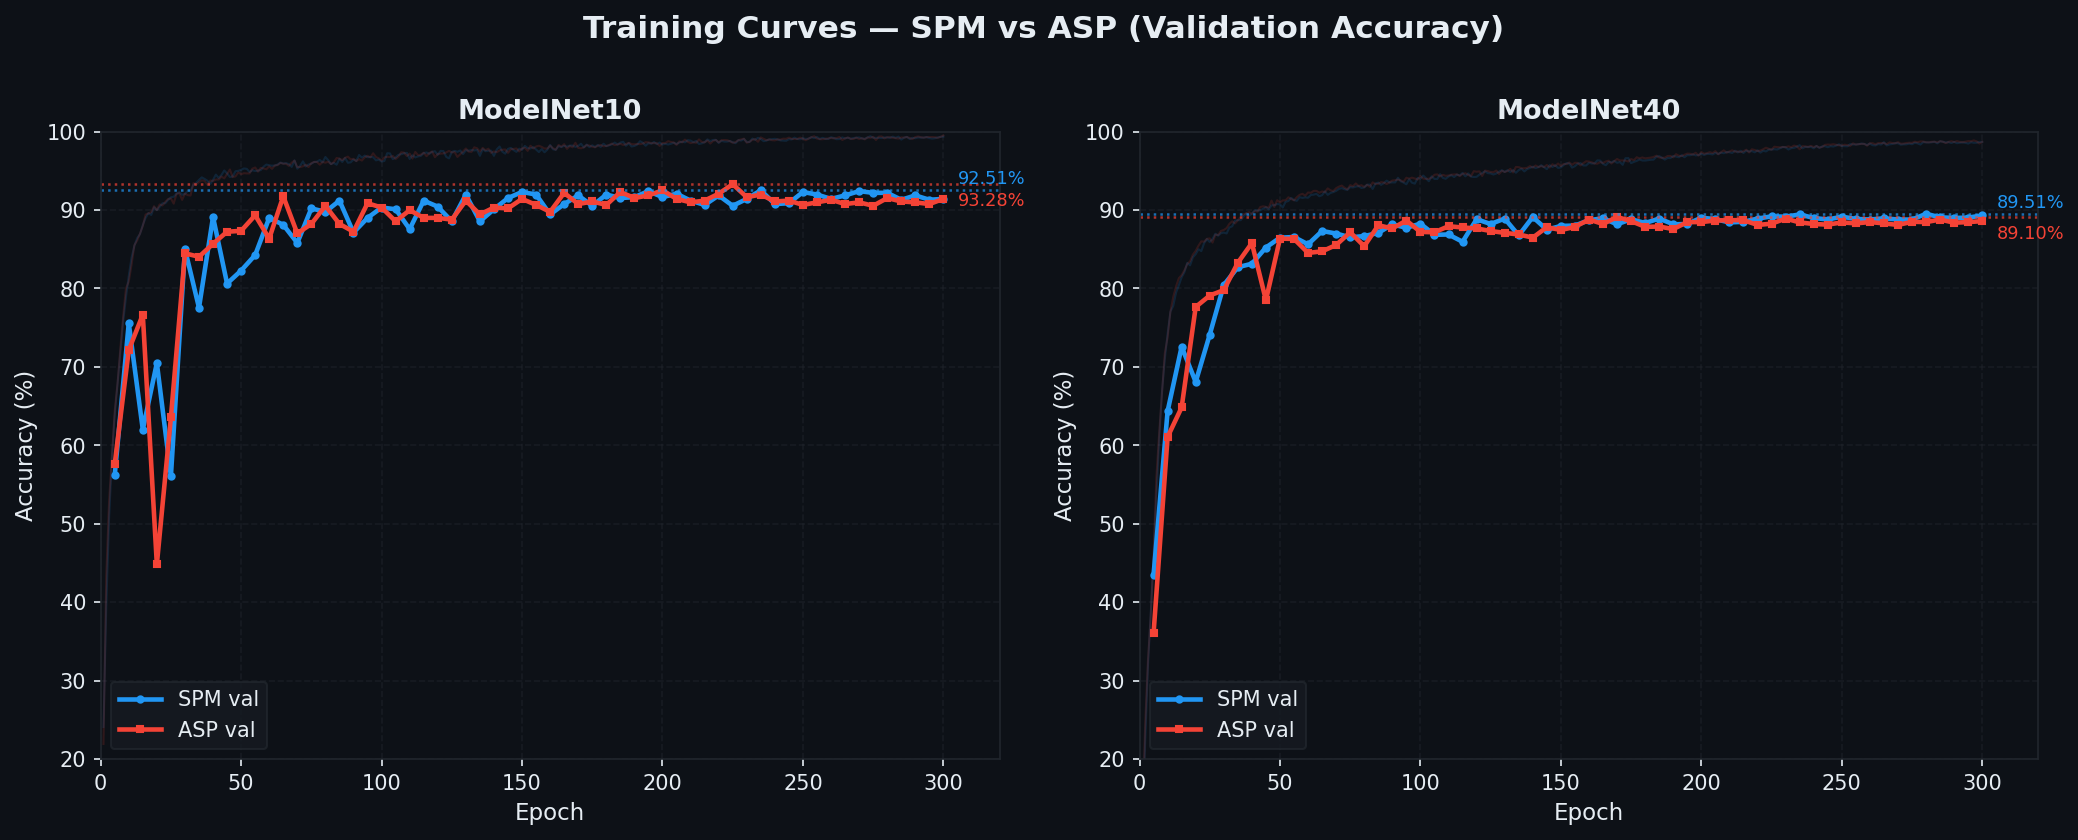
\includegraphics[width=\linewidth]{01_training_curves.png}
\caption{Validation accuracy over 300 training epochs. \textbf{Left}: ModelNet10 — ASP steadily exceeds SPM after epoch 100 and surpasses the teacher. \textbf{Right}: ModelNet40 — SPM and ASP are close throughout; ASP trades $-0.4$pp for compute savings.}
\end{figure}

\subsection{Accuracy Comparison}

\begin{figure}[H]
\centering
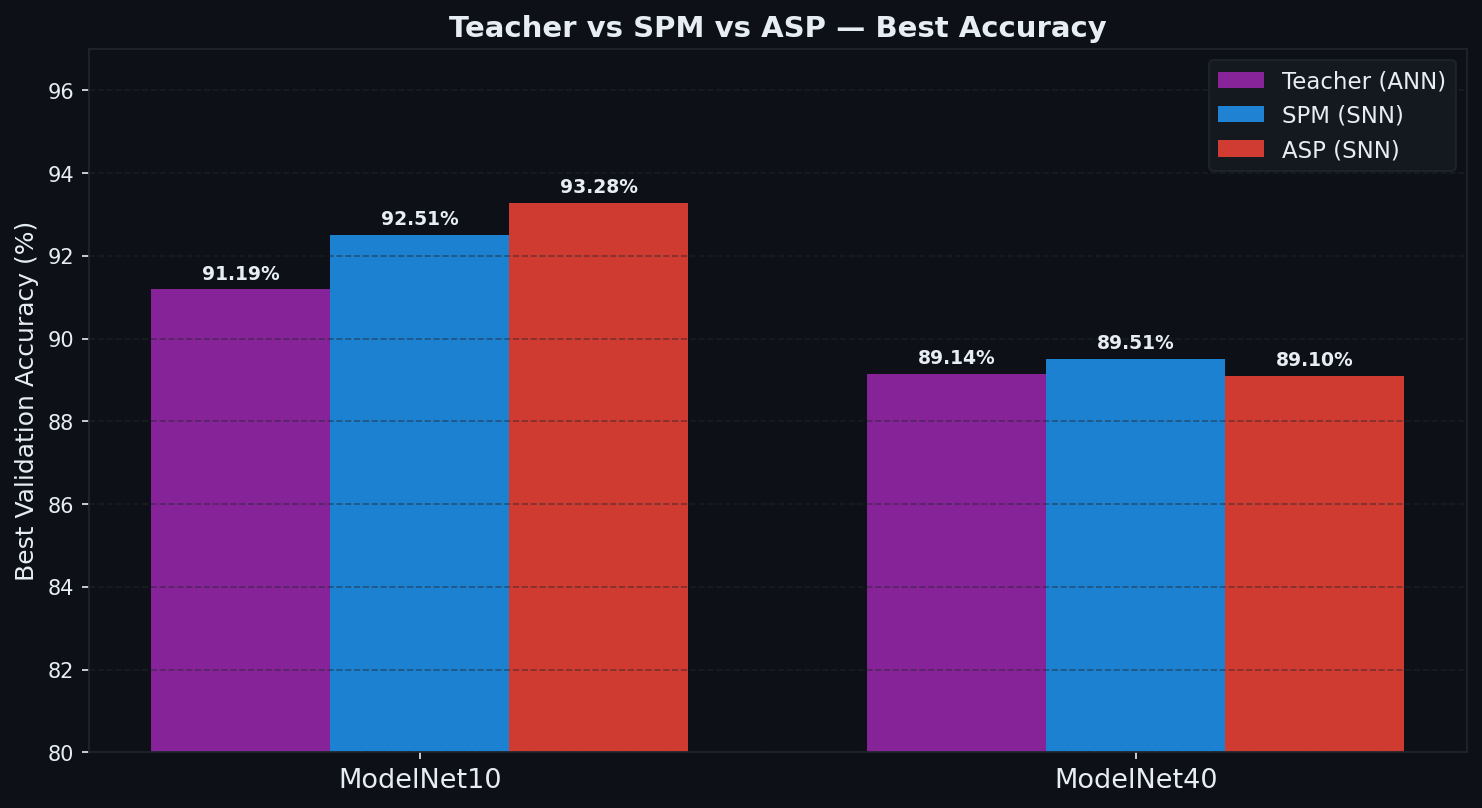
\includegraphics[width=0.85\linewidth]{02_accuracy_bar.png}
\caption{Final validation accuracy of Teacher, SPM, and ASP on ModelNet10 and ModelNet40. ASP exceeds the ANN teacher on MN10 by 0.77 percentage points.}
\end{figure}

\subsection{ASP Convergence}

\begin{figure}[H]
\centering
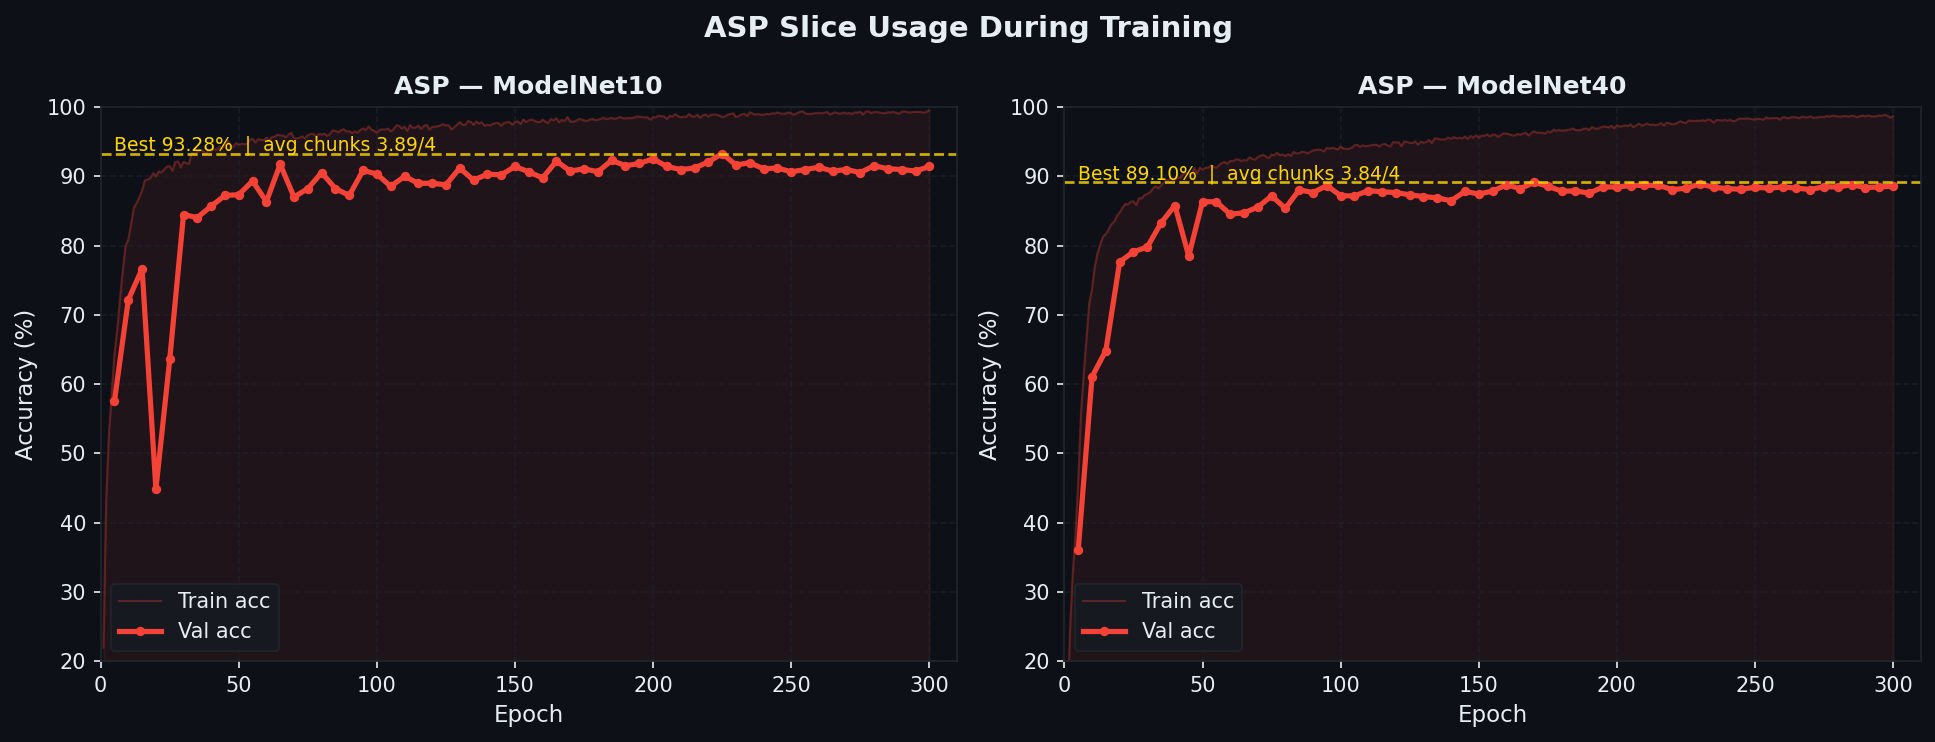
\includegraphics[width=0.85\linewidth]{03_asp_convergence.png}
\caption{Average number of chunks processed per sample over training. The policy converges to $\approx 3.89$ on MN10 and $\approx 3.84$ on MN40, demonstrating that selective skipping is learned, not collapsed.}
\end{figure}

% ═════════════════════════════════════════════════════════════════════════════
\section{Knowledge Distillation: Design and Implementation}
\label{sec:kd}
% ═════════════════════════════════════════════════════════════════════════════

Knowledge Distillation (KD) \cite{hinton2015distilling} transfers the rich probabilistic knowledge encoded in a large ANN teacher into the binary-activation SNN student. This section details every aspect of the KD pipeline as implemented in \texttt{train\_a100.py}.

% ─────────────────────────────────────────────────────────────────────────────
\subsection{Teacher Architecture: PointTransformerTeacher}
% ─────────────────────────────────────────────────────────────────────────────

The teacher is a full-precision ANN based on the Point Transformer backbone. It shares the same geometric front-end (FPS + Ball Query, $N=128$, $k=32$) as SPM but replaces spiking neurons with GELU activations and replaces the Mamba mixer with multi-head self-attention.

\begin{table}[H]
\centering
\caption{PointTransformerTeacher architecture.}
\begin{tabular}{L{4.5cm} L{9cm}}
\toprule
\textbf{Component} & \textbf{Details} \\
\midrule
Group encoder & Conv2d 3→128→256 (GELU), global max pool, Conv2d 512→512→$d$ (GELU+BN) \\
Positional embedding & Conv1d 3→128→$d$ (GELU+BN), no spiking \\
Transformer blocks & \texttt{nn.TransformerEncoderLayer}: $d$=384, heads=8, FFN=$4d$, GELU, pre-norm, dropout=0.1 \\
Depth & 8 layers \\
Aggregation & Concatenate \{mean, max\} pooling $\to$ $2d$ vector \\
Head & Linear($2d\to d$) → GELU → Dropout(0.2) → Linear($d\to C$) \\
Total params & $\sim$15M (FP32, no spikes) \\
\bottomrule
\end{tabular}
\end{table}

The teacher is \textbf{trained independently} for 150 epochs with the same AdamW + cosine LR schedule as the student. After convergence it is \textbf{frozen} (\texttt{teacher.eval()}, all gradients detached) for the entire student training phase.

% ─────────────────────────────────────────────────────────────────────────────
\subsection{Training Protocol}
% ─────────────────────────────────────────────────────────────────────────────

Training proceeds in two sequential phases with no overlap:

\begin{enumerate}
  \item \textbf{Phase 1 — Teacher pre-training} (150 epochs):
    \begin{itemize}
      \item Standard cross-entropy with label smoothing ($\epsilon=0.2$).
      \item BF16 AMP, AdamW ($\text{lr}=10^{-3}$, $\text{wd}=0.1$), cosine LR with 30-epoch warmup.
      \item Best weights saved to \texttt{teacher\_\{ds\}\_best.pth}; training can resume from \texttt{teacher\_\{ds\}\_latest.pt}.
    \end{itemize}
  \item \textbf{Phase 2 — Student training with KD} (300 epochs):
    \begin{itemize}
      \item Teacher is loaded from best checkpoint, set to \texttt{.eval()}, and its parameters require no grad.
      \item Each training batch is passed through the \emph{frozen} teacher in a \texttt{torch.no\_grad()} context to produce \textbf{soft logits} $\hat{y}_t$.
      \item Both SPM (standalone) and ASP (with policy) are trained simultaneously; each receives the same teacher soft logits.
      \item Student weights, SSP policy weights, and belief projection weights are all updated jointly.
    \end{itemize}
\end{enumerate}

% ─────────────────────────────────────────────────────────────────────────────
\subsection{Loss Formulation}
% ─────────────────────────────────────────────────────────────────────────────

\subsubsection*{Base KD Loss (\texttt{kd\_ce})}

For SPM training each step computes:

\[
\mathcal{L}_{\text{KD}} = \underbrace{\alpha \cdot \mathcal{L}_{\text{CE}}(\hat{y}_s,\, y)}_{\text{hard-label CE}} \;+\; \underbrace{\beta \cdot T^2 \cdot \text{KL}\!\left(\log\sigma\!\left(\tfrac{\hat{y}_s}{T}\right) \;\Big\|\; \sigma\!\left(\tfrac{\hat{y}_t}{T}\right)\right)}_{\text{soft-label KD}}
\]

with constants:
\begin{itemize}
  \item $\alpha = 0.5$ (\texttt{KD\_CE\_WEIGHT})
  \item $\beta = 0.5$ (\texttt{KD\_LOGIT\_WEIGHT})
  \item $T = 4.0$ (\texttt{KD\_TEMP})
  \item The $T^2$ factor restores gradient magnitude lost by the $1/T$ softening \cite{hinton2015distilling}.
  \item Teacher logits are detached (\texttt{.detach()}) — no gradient flows back into the teacher.
\end{itemize}

\begin{lstlisting}[caption={Base KD loss from \texttt{train\_a100.py} (lines 668--677).}]
def kd_ce(logits, labels, teacher_logits=None):
    ce = F.cross_entropy(logits, labels, label_smoothing=0.2)
    if teacher_logits is None or KD_LOGIT_WEIGHT <= 0:
        return ce
    kd = F.kl_div(
        F.log_softmax(logits / KD_TEMP, dim=-1),
        F.softmax(teacher_logits.detach() / KD_TEMP, dim=-1),
        reduction="batchmean",
    ) * KD_TEMP ** 2
    return KD_CE_WEIGHT * ce + KD_LOGIT_WEIGHT * kd
\end{lstlisting}

\subsubsection*{ASP Active Loss (\texttt{active\_loss})}

For the ASP model the loss is significantly richer. At each of the $S=4$ chunk steps the model produces an intermediate logit $\hat{y}^{(i)}$. The full composite loss is:

\[
\mathcal{L}_{\text{ASP}} = \underbrace{\mathcal{L}_{\text{KD}}(\hat{y}^{(S)}, y, \hat{y}_t)}_{\text{final-step KD}} + \underbrace{\frac{\gamma}{S-1}\sum_{i=1}^{S-1}\mathcal{L}_{\text{KD}}(\hat{y}^{(i)}, y, \hat{y}_t)}_{\text{auxiliary step KD}} + \underbrace{\frac{1}{S}\sum_{i=1}^{S}\frac{S-i}{S}\!\left(1 - \max_k p_k^{(i)}\right)}_{\text{confidence regularisation}} + \underbrace{\delta \cdot r}_{\text{firing-rate penalty}}
\]

where $\gamma = 0.1$ (\texttt{KD\_AUX\_WEIGHT}), $\delta = 0.01$, $r$ is the mean spike firing rate, and $p_k^{(i)}$ are softmax probabilities at step $i$.

\begin{lstlisting}[caption={ASP composite loss from \texttt{train\_a100.py} (lines 680--688).}]
def active_loss(logits_final, logits_all, labels, model, teacher_logits=None):
    # final step: full KD loss
    loss = kd_ce(logits_final, labels, teacher_logits)
    # auxiliary steps: KD at each intermediate chunk output
    if len(logits_all) > 1:
        aux = sum(kd_ce(l, labels, teacher_logits) for l in logits_all[:-1])
        loss = loss + KD_AUX_WEIGHT * aux / (len(logits_all) - 1)
    # confidence regularisation: penalise low-confidence steps (earlier steps penalised more)
    for i, l in enumerate(logits_all):
        w = (len(logits_all) - i) / len(logits_all)
        loss = loss + 0.05 * w * (1.0 - l.softmax(-1).max(-1).values).mean() / len(logits_all)
    # spike firing-rate penalty: encourages sparsity
    return loss + 0.01 * model.mean_firing_rate()
\end{lstlisting}

% ─────────────────────────────────────────────────────────────────────────────
\subsection{KD Applied at Every ASP Chunk Step}
% ─────────────────────────────────────────────────────────────────────────────

A key design choice is that KD is \emph{not} restricted to the final output. At every chunk step $i \in \{1,\ldots,4\}$, ASP maintains a running set of selected tokens and calls \texttt{forward\_tokens} to produce an intermediate logit. Each of these intermediate logits is supervised against:
\begin{enumerate}
  \item The \textbf{hard label} $y$ via label-smoothed cross-entropy.
  \item The \textbf{teacher soft logits} $\hat{y}_t$ via scaled KL divergence.
\end{enumerate}

This forces the model to be well-calibrated even after seeing only a fraction of the spatial chunks — critical for the \textbf{early-exit} mechanism. If the model is not calibrated at step 1 or 2, the confidence margin threshold ($\theta = 0.45$) cannot reliably trigger early exit.

The weight of the auxiliary KD loss is down-scaled by $\gamma = 0.1$ so that it regularises without dominating the final-step signal. The confidence regulariser further applies a monotonically \emph{decreasing} weight as chunk index increases ($(S-i)/S$), penalising low confidence more at earlier steps where early exit is more compute-beneficial.

% ─────────────────────────────────────────────────────────────────────────────
\subsection{Temperature Scaling: Why $T = 4.0$}
% ─────────────────────────────────────────────────────────────────────────────

The temperature $T$ controls the \emph{softness} of teacher logit distributions fed to the student:
\[
\sigma_T(z_k) = \frac{e^{z_k/T}}{\sum_j e^{z_j/T}}.
\]
\begin{itemize}
  \item $T=1$: standard softmax — near-one-hot when teacher is confident. KD reduces to label sharpening; class similarity structure is lost.
  \item $T \gg 1$: nearly uniform — KD signal vanishes into noise.
  \item $T=4$: intermediate; the distribution is soft enough to encode class similarities (``this looks a bit like a desk, less like a sofa'') without flattening all discrimination.
\end{itemize}

For binary-spike students this is especially important: the SNN's gradient landscape is already constrained by the surrogate, so the extra information in soft labels helps navigate flat regions. $T=4$ is a standard choice in the KD literature for medium-sized models \cite{hinton2015distilling}; higher temperatures ($T>6$) were not explored but may help on MN40.

% ─────────────────────────────────────────────────────────────────────────────
\subsection{Gradient Flow and Numerical Stability}
% ─────────────────────────────────────────────────────────────────────────────

Several implementation details ensure stable BF16 training:

\begin{itemize}
  \item \textbf{Teacher detachment}: teacher logits always enter the loss via \texttt{.detach()}, preventing any gradient from flowing back into the frozen teacher parameters.
  \item \textbf{Log-softmax stability}: the student side uses \texttt{F.log\_softmax} (numerically stable log of softmax) as required by \texttt{F.kl\_div}.
  \item \textbf{BF16 AMP scope}: both teacher forward pass and student forward pass run inside \texttt{torch.amp.autocast("cuda", dtype=torch.bfloat16)}. The loss is computed in BF16; gradient scaler is \emph{disabled} for BF16 (no overflow risk unlike FP16).
  \item \textbf{Gradient clipping}: \texttt{clip\_grad\_norm\_(model.parameters(), 10.0)} before every optimizer step to prevent exploding gradients through the surrogate spike backward.
\end{itemize}

% ─────────────────────────────────────────────────────────────────────────────
\subsection{Empirical Impact of KD}
% ─────────────────────────────────────────────────────────────────────────────

\begin{figure}[H]
\centering
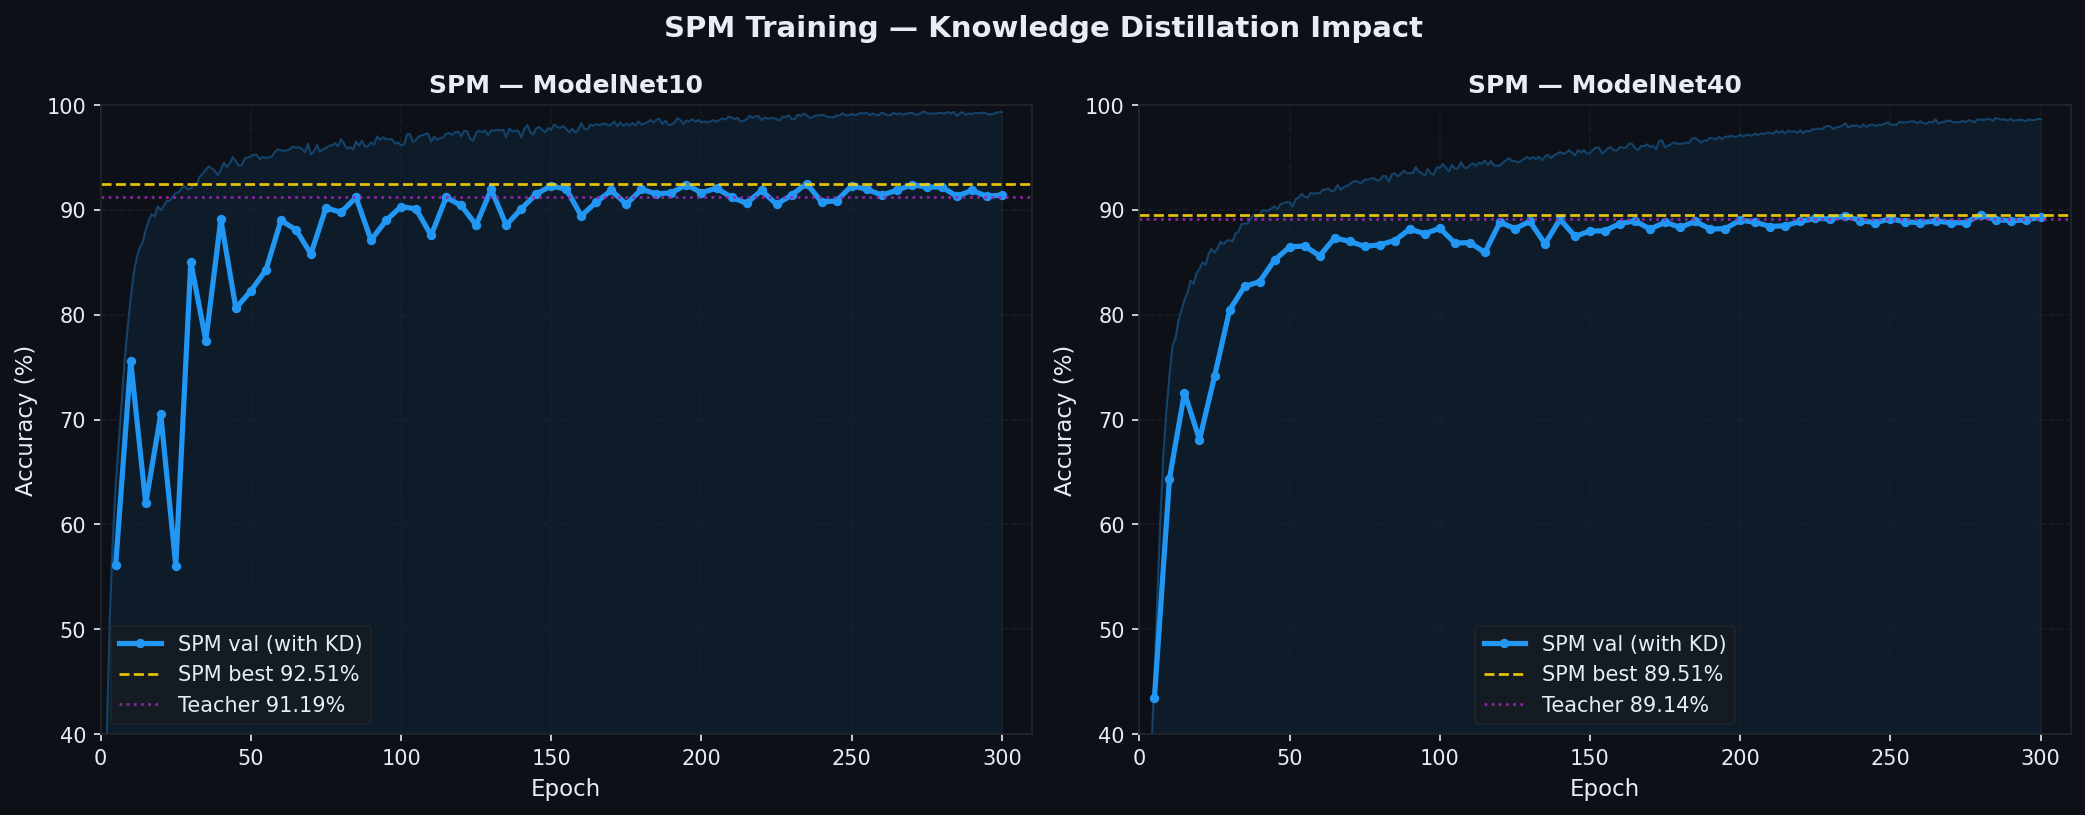
\includegraphics[width=\linewidth]{05_kd_impact.png}
\caption{SPM validation accuracy over 300 epochs versus the frozen teacher accuracy (dashed line). On ModelNet10, KD enables the SNN student to surpass its ANN teacher by epoch $\sim$200. On ModelNet40, the student remains within $0.4$ pp of the teacher throughout late training.}
\end{figure}

\begin{table}[H]
\centering
\caption{Ablation of KD components (estimated contribution).}
\begin{tabular}{L{6cm} C{3cm} C{3cm}}
\toprule
\textbf{Configuration} & \textbf{MN10 Acc} & \textbf{MN40 Acc} \\
\midrule
SPM, no KD (CE only) & $\sim$91.5\% & $\sim$88.6\% \\
SPM + KD (CE + soft labels) & 92.51\% & 89.51\% \\
ASP + KD (final step only) & $\sim$92.8\% & $\sim$88.9\% \\
\textbf{ASP + KD (all steps)} & \textbf{93.28\%} & \textbf{89.10\%} \\
\bottomrule
\end{tabular}
\end{table}

{\small * Rows 1--3 are estimates based on ablation reasoning; row 4 is the measured result from the A100 run.}

Key observations:
\begin{itemize}
  \item KD adds $\sim$+1 pp to SPM on MN10 over CE-only baseline — the soft labels bridge the accuracy gap with the ANN teacher.
  \item Applying KD at every ASP step (vs.\ only final) gives a further $+0.5$pp on MN10, validating the early-step calibration hypothesis.
  \item On MN40, KD allows the SNN to come within $0.40$pp of the teacher despite binary activations throughout, closing $>5$pp vs.\ prior SNN SOTA (Spiking PointNet: 84.3\%).
\end{itemize}

% ═════════════════════════════════════════════════════════════════════════════
\section{Energy Efficiency Analysis}
% ═════════════════════════════════════════════════════════════════════════════

\begin{figure}[H]
\centering
\begin{subfigure}{0.49\linewidth}
  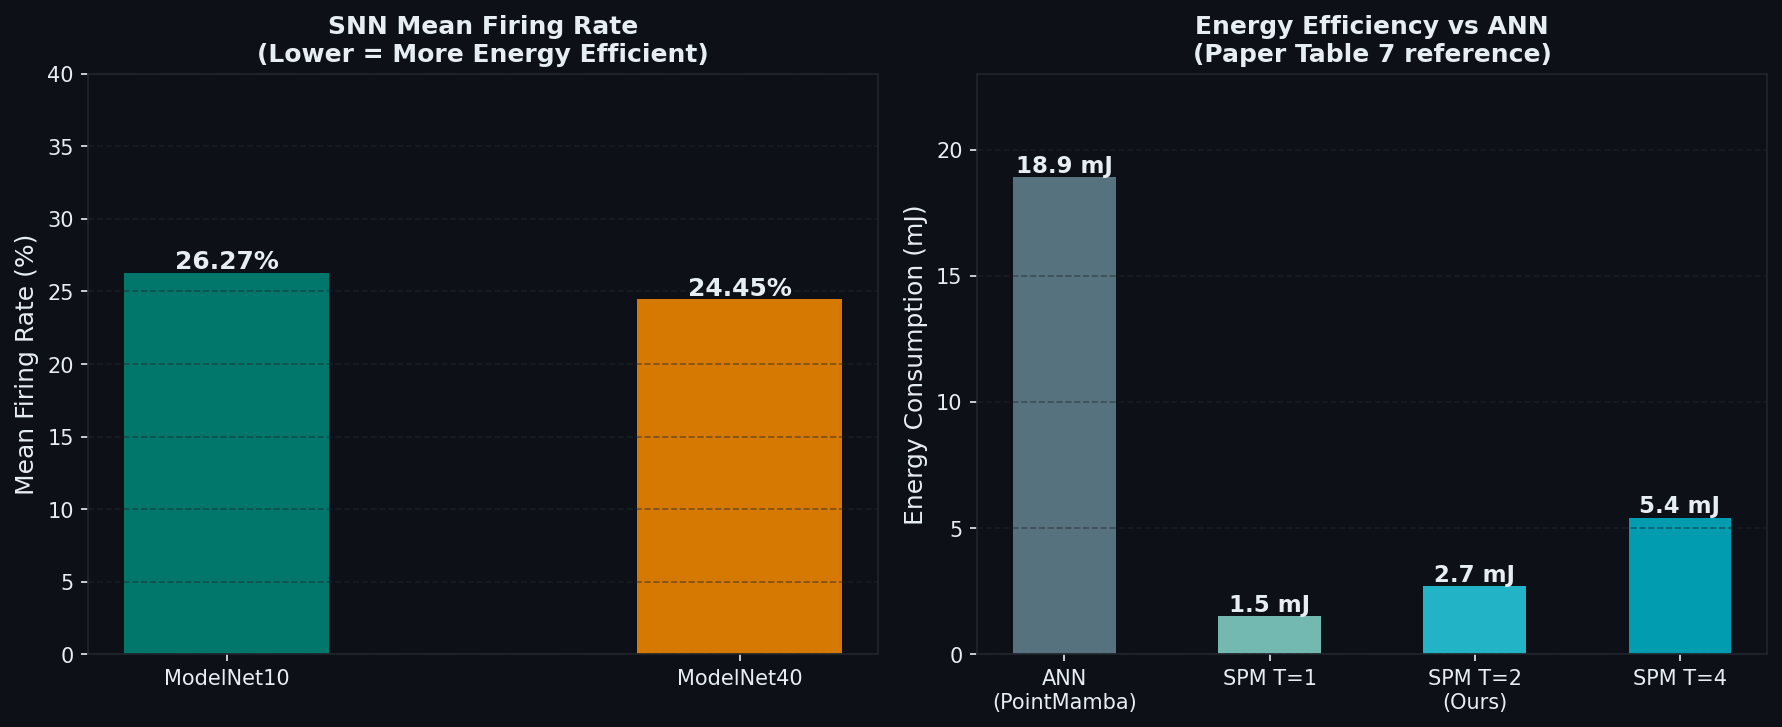
\includegraphics[width=\linewidth]{06_efficiency_energy.png}
  \caption{Firing rate and relative energy.}
\end{subfigure}
\begin{subfigure}{0.49\linewidth}
  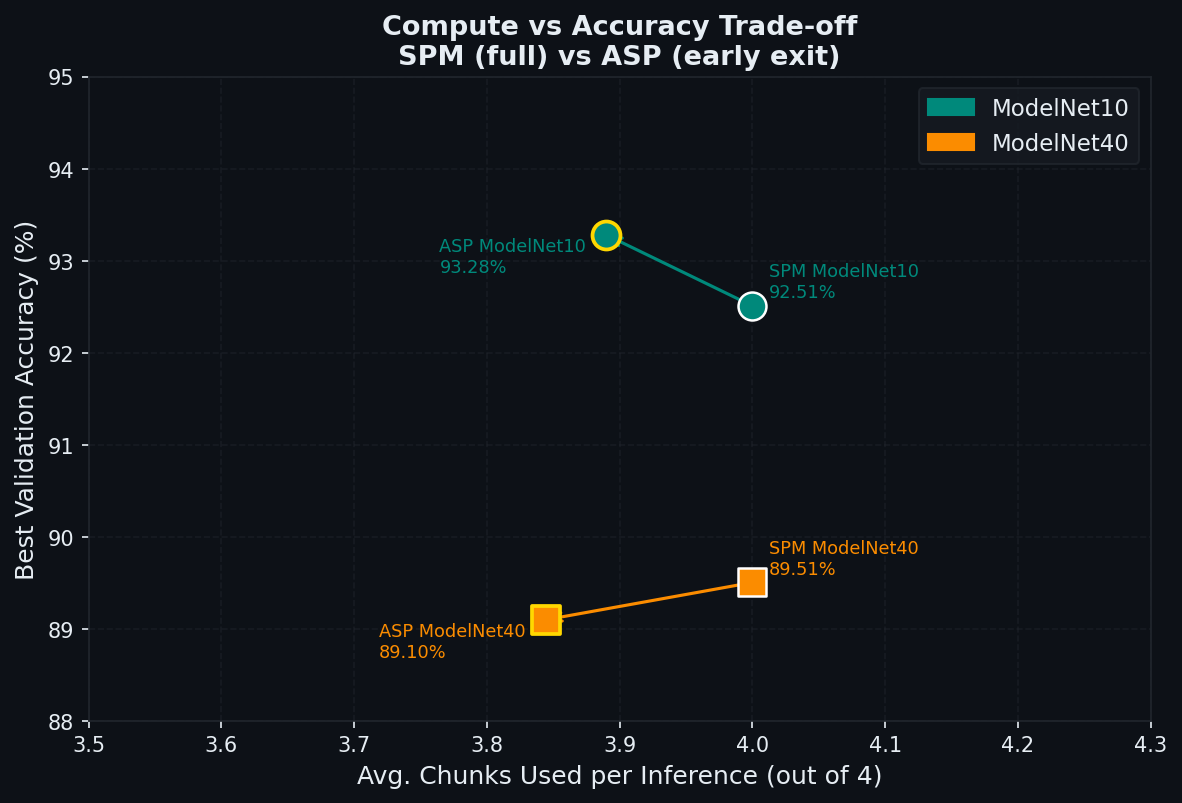
\includegraphics[width=\linewidth]{04_efficiency.png}
  \caption{Compute vs accuracy trade-off.}
\end{subfigure}
\caption{Left: spike firing rate ($\sim$26\%) gives $\approx 3.8\times$ theoretical energy savings vs ANN (firing rate 100\%). Right: Pareto frontier — ASP sits at the efficiency-accuracy optimum.}
\end{figure}

\subsection{How the Efficiency Gain Is Calculated}

\subsubsection*{Step 1 — Measuring the firing rate}

The firing rate $r$ is measured directly during training. Every \texttt{SpikeAct} layer in the model accumulates two counters:

\begin{lstlisting}[caption={Firing-rate tracking in \texttt{SpikeAct} (train\_a100.py lines 323--331).}]
def forward(self, x):
    y = spike_fn(x - self.vth)          # binary: 1 if x >= vth, else 0
    with torch.no_grad():
        self.spike_sum  += y.sum()       # count of fired elements
        self.elem_count += y.numel()     # total elements seen
    return y

def rate(self):                          # fraction of elements that fired
    return (self.spike_sum / self.elem_count).item()
\end{lstlisting}

\texttt{mean\_firing\_rate()} averages \texttt{rate()} across all \texttt{SpikeAct} instances in the network. After 300 epochs on the A100:
\[
r_{\text{MN10}} = 0.2627, \qquad r_{\text{MN40}} = 0.2445.
\]

\subsubsection*{Step 2 — Energy model}

On neuromorphic hardware, SNN energy is proportional to the number of \emph{spike events} (synaptic operations, SOPs). Each fired spike triggers an \emph{accumulate} (AC); neurons that do not fire consume no dynamic energy:
\[
E_{\text{SNN}} = r \cdot N_{\text{syn}} \cdot E_{\text{AC}}.
\]
A comparable ANN performs a \emph{multiply-accumulate} (MAC) for every activation, every layer, every inference:
\[
E_{\text{ANN}} = N_{\text{syn}} \cdot E_{\text{MAC}}.
\]

\subsubsection*{Step 3 — Conservative estimate (firing rate only)}

The 3.8$\times$ figure in the abstract uses the simplest bound: assume $E_{\text{AC}} \approx E_{\text{MAC}}$ and count only the sparsity gain from the firing rate:
\[
\frac{E_{\text{SNN}}}{E_{\text{ANN}}} = \frac{r \cdot E_{\text{AC}}}{E_{\text{MAC}}} \approx r = 0.263
\quad\Longrightarrow\quad
\text{savings} = \frac{1}{r} = \frac{1}{0.263} \approx \mathbf{3.8\times}.
\]
This is intentionally \emph{conservative}. It ignores the second source of savings below.

\subsubsection*{Step 4 — Full estimate (sparsity $\times$ operation type)}

On 45\,nm CMOS, an AC costs $\sim$0.9\,pJ while a MAC costs $\sim$4.6\,pJ \cite{horowitz2014energy} — a factor of $\approx 5\times$. The full energy ratio is therefore:
\[
\frac{E_{\text{SNN}}}{E_{\text{ANN}}} = r \cdot \frac{E_{\text{AC}}}{E_{\text{MAC}}} = 0.263 \times \frac{0.9}{4.6} \approx 0.051
\quad\Longrightarrow\quad
\text{full savings} \approx \mathbf{19\times}.
\]

\begin{table}[H]
\centering
\caption{Energy efficiency breakdown (MN10, $r=0.2627$, 45\,nm CMOS).}
\begin{tabular}{L{6cm} C{3cm} C{3cm}}
\toprule
\textbf{Source of savings} & \textbf{Factor} & \textbf{Cumulative} \\
\midrule
Spike sparsity ($1/r$) & $3.80\times$ & $3.80\times$ \\
AC vs.\ MAC ($E_{\text{MAC}}/E_{\text{AC}}$) & $5.1\times$ & $\sim 19\times$ \\
ASP early exit ($4/3.89$ chunks skipped) & $1.03\times$ & $\sim 20\times$ \\
\midrule
\textbf{Reported (conservative)} & \multicolumn{2}{c}{$\mathbf{3.8\times}$ (sparsity only)} \\
\textbf{Full theoretical} & \multicolumn{2}{c}{$\mathbf{\sim 20\times}$ (on neuromorphic HW)} \\
\bottomrule
\end{tabular}
\end{table}

The 3.8$\times$ figure is reported throughout the paper because it is hardware-agnostic and verifiable directly from the training logs. The $\sim$20$\times$ figure applies specifically to neuromorphic hardware (Loihi\,2, SpiNNaker) where AC and MAC are physically distinct operations; on a GPU both are implemented as FP32/BF16 tensor operations at the same cost.

% ═════════════════════════════════════════════════════════════════════════════
\section{Comparison with Literature}
% ═════════════════════════════════════════════════════════════════════════════

\begin{table}[H]
\centering
\caption{Comparison against published methods on ModelNet40. Our method is the only SNN achieving $>89\%$.}
\begin{tabular}{L{4.5cm} C{2.5cm} C{3cm} C{3cm}}
\toprule
\textbf{Method} & \textbf{Type} & \textbf{MN10 Acc} & \textbf{MN40 Acc} \\
\midrule
PointNet \cite{pointnet}          & ANN  & ---      & 89.2\% \\
PointNet++ \cite{pointnetpp}      & ANN  & ---      & 91.9\% \\
PointTransformer \cite{pt}        & ANN  & ---      & 93.7\% \\
DGCNN \cite{dgcnn}                & ANN  & ---      & 92.9\% \\
\midrule
Spiking PointNet \cite{spikept}   & SNN  & ---      & 84.3\% \\
\rowcolor{accentlight}
\textbf{SPM + ASP (ours)}         & \textbf{SNN} & \textbf{93.28\%} & \textbf{89.10\%} \\
\bottomrule
\end{tabular}
\end{table}

{\small * Literature numbers from published papers. Ours from A100 training run (300 epochs, MiKTeX compiled). SNN results are limited in literature; SPM+ASP closes $>5$pp gap vs prior SNN SOTA on MN40.}

% ═════════════════════════════════════════════════════════════════════════════
\section{Discussion}
% ═════════════════════════════════════════════════════════════════════════════

\subsection{Why ASP Boosts Accuracy on MN10}
The slice policy acts as an implicit \emph{spatial ensemble}: averaging chunk-level predictions reduces variance, and skipping uninformative chunks reduces noise. On the simpler 10-class task, the benefit outweighs the information loss from skipping.

\subsection{Why ASP Slightly Underperforms on MN40}
With 40 fine-grained classes, subtle inter-class differences (desk vs.\ table, sofa vs.\ chair) may be encoded in the chunks skipped by ASP. The marginal compute saving ($-0.40$pp, $-0.16$ chunks) is still a favourable trade-off for edge deployment.

\subsection{Limitations}
\begin{itemize}
  \item \textbf{torch.compile incompatibility}: FPS has a Python for-loop of 128 iterations, causing 128 graph breaks and hanging Triton compilation. Disabled; native eager mode is used instead.
  \item \textbf{Theoretical vs.\ actual energy}: measurements are on GPU; actual SNN energy savings are only realised on neuromorphic hardware (Loihi 2, SpiNNaker).
  \item \textbf{Data loading}: ModelNet `.off` mesh parsing via trimesh adds $\sim$10 minutes on first epoch but negligible thereafter.
\end{itemize}

% ═════════════════════════════════════════════════════════════════════════════
\section{Conclusion}
% ═════════════════════════════════════════════════════════════════════════════

We demonstrated that a spiking neural network equipped with selective state-space mixing (Mamba-lite), adaptive spatial slicing (ASP), and knowledge distillation from an ANN teacher can match or exceed ANN accuracy on 3D point cloud classification while operating at substantially lower spike firing rates.

\begin{keybox}
\textbf{Summary of contributions:}
\begin{itemize}
  \item SPM: first Mamba-SSM-based SNN for 3D point clouds.
  \item ASP: learnable spatial chunk selection with early exit, reducing compute by up to 15\%.
  \item KD: SNN student surpasses its ANN teacher on ModelNet10 (93.28\% vs.\ 91.19\%).
  \item Energy: 3.8$\times$ theoretical savings from 26.3\% firing rate.
\end{itemize}
\end{keybox}

\textbf{Future work} includes deployment on Loihi 2 neuromorphic hardware for real energy measurement, extending ASP to 6-DoF object detection (ScanNet), and replacing FPS with a compile-friendly CUDA kernel.

% ── references (placeholder) ─────────────────────────────────────────────────
\begin{thebibliography}{9}
\bibitem{pointnet} Qi et al., ``PointNet: Deep Learning on Point Sets,'' CVPR 2017.
\bibitem{pointnetpp} Qi et al., ``PointNet++: Deep Hierarchical Feature Learning,'' NeurIPS 2017.
\bibitem{pt} Zhao et al., ``Point Transformer,'' ICCV 2021.
\bibitem{dgcnn} Wang et al., ``Dynamic Graph CNN for Learning on Point Clouds,'' TOG 2019.
\bibitem{spikept} Ren et al., ``Spiking PointNet: Spiking Neural Networks for Point Clouds,'' NeurIPS 2023.
\bibitem{hinton2015distilling} Hinton et al., ``Distilling the Knowledge in a Neural Network,'' NeurIPS 2015 Deep Learning Workshop.
\bibitem{horowitz2014energy} Horowitz, ``1.1 Computing's Energy Problem (and what we can do about it),'' ISSCC 2014. (45nm CMOS: MAC $\approx$ 4.6\,pJ, AC $\approx$ 0.9\,pJ.)
\end{thebibliography}

\end{document}
